\documentclass[a4paper,twocolumn,12pt]{article}
\usepackage[utf8]{inputenc}
\usepackage[MeX]{polski}
\usepackage{fullpage}
\usepackage{tikz}
\usetikzlibrary{calc,shapes,shapes.multipart, arrows}
\usepackage{pgfplots}
\pgfplotsset{compat=1.8}
\usepackage{hyperref}

% ;;;;;;;;; colors ;;;;;;;;;;;;

\definecolor{Board}{RGB}{60,145,143}
\definecolor{DoubleWordBonus}{RGB}{239,174,154}
\definecolor{DoubleLetterBonus}{RGB}{141,201,240}
\definecolor{TripleLetterBonus}{RGB}{54,156,219}
\definecolor{Tile}{RGB}{247,225,190}
\definecolor{UniGreen}{RGB}{0,100,200}

% ;;;;;;;;;;;;;;;;;;;;;;;;;;;;;;;;

\title{\LARGE{Sztuczna inteligencja grająca w~Scrabble} \\ \vspace{2mm} \large{Koncepcja implementacji - dane, struktury danych, algorytmy}}
\author{Jakub Turek}
\date{\today}

\begin{document}

\maketitle

\begin{abstract}
Celem artykułu jest opisanie zbioru koncepcji, które posłużą do implementacji algorytmu sztucznej inteligencji grającego w~grę Scrabble w~języku polskim. Artykuł analizuje i~porównuje dane zawarte w~dwóch głównych słownikach wyrazów do gier dla języka polskiego, przedstawia dane statystyczne ułatwiające wprowadzanie heurystyk do algorytmu, a~także opisuje metody niezbędne do wyznaczania wszystkich możliwych kombinacji ruchów w~danej turze. Autor omawia również podział rozgrywki na fazy gry i~przybliża podejście, które pozwala uzyskiwać najlepsze wyniki dla każdej fazy gry.
\end{abstract}

\section*{Wstęp}

Scrabble to ,,gra słowna polegająca na układaniu na określonej planszy wyrazów z~losowanych liter''\footnote{Wielki słownik ortograficzny - PWN 2003, 2006, 2008 - E. Polański}. Jest to bardzo ogólna definicja, którą należy uściślić. Scrabble jest grą przeznaczoną dla 2-4 osób. Akcesoriami do gry są: kwadratowa plansza o~stałym rozmiarze $15 \times 15$, torebka wypełniona płytkami, na których nadrukowane są litery oraz ich wartości punktowe, a~także stojaki, na których gracze umieszczają płytki, którymi w~danej chwili dysponują.

Gra rozgrywana jest w~turach. Zadaniem graczy jest układanie wyrazów na planszy, w~taki sposób aby tworzyły one poprawne słowa w~języku, w~którym prowadzona jest rozgrywka, w~układzie krzyżówkowym. Układ krzyżówkowy został przedstawiony na rysunkach \ref{fig:crossword_first} oraz \ref{fig:crossword_second}:

\begin{description}
 \item [Rysunek \ref{fig:crossword_first}] Pokazuje sytuację początkową obrazującą pewien moment rozgrywki.
 \item [Rysunek \ref{fig:crossword_second}] Pokazuje poprawny ruch zawodnika, który powoduje powstanie więcej niż jednego słowa. Wszystkie wyrazy utworzone przez jeden ruch muszą być poprawne. W~podanym przykładzie słowa ,,za'' i~,,masz'' są poprawne.
\end{description}

\begin{figure}[ht!]
	\begin{center}
			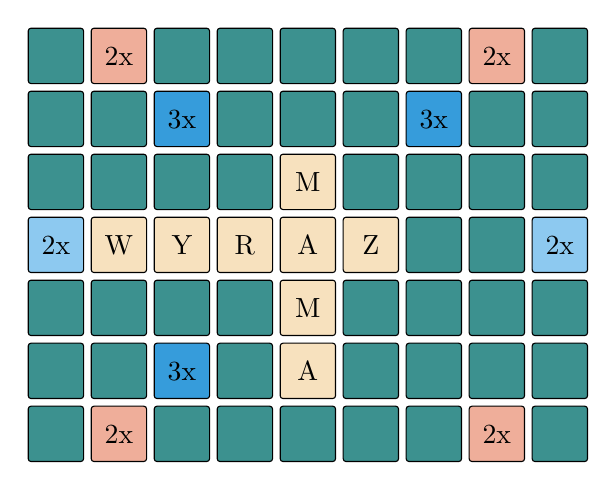
\begin{tikzpicture}
			\tikzstyle{every node}=[draw, shape=rectangle, rounded corners = 1pt, minimum width = 20pt, minimum height = 20pt, align=center, text height = 7pt];
			\node [fill=Board] at (-0.8, 0) {};
			\node [fill=DoubleWordBonus] at (0, 0) {2x};
			\node [fill=Board] at (0.8, 0) {};
			\node [fill=Board] at (1.6, 0) {};
			\node [fill=Board] at (2.4, 0) {};
			\node [fill=Board] at (3.2, 0) {};
			\node [fill=Board] at (4.0, 0) {};
			\node [fill=DoubleWordBonus] at (4.8, 0) {2x};
			\node [fill=Board] at (5.6, 0) {};
			\node [fill=Board] at (-.8, -.8) {};
			\node [fill=Board] at (0, -.8) {};
			\node [fill=TripleLetterBonus] at (0.8, -.8) {3x};
			\node [fill=Board] at (1.6, -.8) {};
			\node [fill=Board] at (2.4, -.8) {};
			\node [fill=Board] at (3.2, -.8) {};
			\node [fill=TripleLetterBonus] at (4.0, -.8) {3x};
			\node [fill=Board] at (4.8, -.8) {};
			\node [fill=Board] at (5.6, -.8) {};
			\node [fill=Board] at (-.8, -1.6) {};
			\node [fill=Board] at (0, -1.6) {};
			\node [fill=Board] at (0.8, -1.6) {};
			\node [fill=Board] at (1.6, -1.6) {};
			\node [fill=Tile] at (2.4, -1.6) {M};
			\node [fill=Board] at (3.2, -1.6) {};
			\node [fill=Board] at (4.0, -1.6) {};
			\node [fill=Board] at (4.8, -1.6) {};
			\node [fill=Board] at (5.6, -1.6) {};
			\node [fill=DoubleLetterBonus] at (-.8, -2.4) {2x};
			\node [fill=Tile] at (0, -2.4) {W};
			\node [fill=Tile] at (.8, -2.4) {Y};
			\node [fill=Tile] at (1.6, -2.4) {R};
			\node [fill=Tile] at (2.4, -2.4) {A};
			\node [fill=Tile] at (3.2, -2.4) {Z};
			\node [fill=Board] at (4.0, -2.4) {};
			\node [fill=Board] at (4.8, -2.4) {};
			\node [fill=DoubleLetterBonus] at (5.6, -2.4) {2x};
			\node [fill=Board] at (-.8, -3.2) {};
			\node [fill=Board] at (0, -3.2) {};
			\node [fill=Board] at (0.8, -3.2) {};
			\node [fill=Board] at (1.6, -3.2) {};
			\node [fill=Tile] at (2.4, -3.2) {M};
			\node [fill=Board] at (3.2, -3.2) {};
			\node [fill=Board] at (4.0, -3.2) {};
			\node [fill=Board] at (4.8, -3.2) {};
			\node [fill=Board] at (5.6, -3.2) {};
			\node [fill=Board] at (-.8, -4.0) {};
			\node [fill=Board] at (0, -4.0) {};
			\node [fill=TripleLetterBonus] at (0.8, -4.0) {3x};
			\node [fill=Board] at (1.6, -4.0) {};
			\node [fill=Tile] at (2.4, -4.0) {A};
			\node [fill=Board] at (3.2, -4.0) {};
			\node [fill=Board] at (4.0, -4.0) {};
			\node [fill=Board] at (4.8, -4.0) {};
			\node [fill=Board] at (5.6, -4.0) {};
			\node [fill=Board] at (-.8, -4.8) {};
			\node [fill=DoubleWordBonus] at (0, -4.8) {2x};
			\node [fill=Board] at (0.8, -4.8) {};
			\node [fill=Board] at (1.6, -4.8) {};
			\node [fill=Board] at (2.4, -4.8) {};
			\node [fill=Board] at (3.2, -4.8) {};
			\node [fill=Board] at (4.0, -4.8) {};
			\node [fill=DoubleWordBonus] at (4.8, -4.8) {2x};
			\node [fill=Board] at (5.6, -4.8) {};
		\end{tikzpicture}
		\caption{Fragment planszy. Gracze ułożyli kolejno słowa: ,,wyraz'' oraz ''mama''.}
		\label{fig:crossword_first}
	\end{center}
\end{figure}

\begin{figure}[ht!]
	\begin{center}
			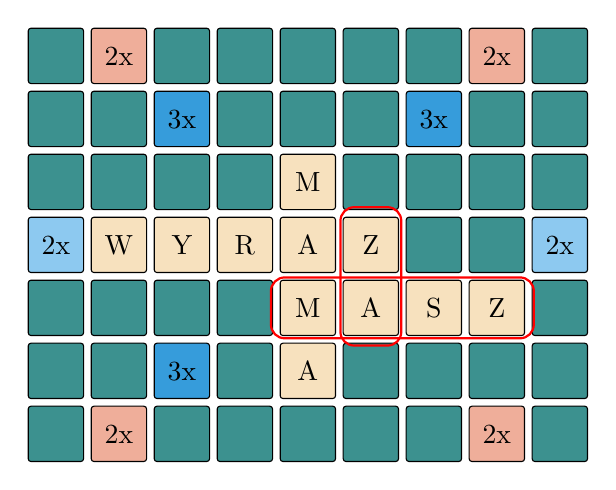
\begin{tikzpicture}
			\tikzstyle{every node}=[draw, shape=rectangle, rounded corners = 1pt, minimum width = 20pt, minimum height = 20pt, align=center, text height = 7pt];
			\node [fill=Board] at (-0.8, 0) {};
			\node [fill=DoubleWordBonus] at (0, 0) {2x};
			\node [fill=Board] at (0.8, 0) {};
			\node [fill=Board] at (1.6, 0) {};
			\node [fill=Board] at (2.4, 0) {};
			\node [fill=Board] at (3.2, 0) {};
			\node [fill=Board] at (4.0, 0) {};
			\node [fill=DoubleWordBonus] at (4.8, 0) {2x};
			\node [fill=Board] at (5.6, 0) {};
			\node [fill=Board] at (-.8, -.8) {};
			\node [fill=Board] at (0, -.8) {};
			\node [fill=TripleLetterBonus] at (0.8, -.8) {3x};
			\node [fill=Board] at (1.6, -.8) {};
			\node [fill=Board] at (2.4, -.8) {};
			\node [fill=Board] at (3.2, -.8) {};
			\node [fill=TripleLetterBonus] at (4.0, -.8) {3x};
			\node [fill=Board] at (4.8, -.8) {};
			\node [fill=Board] at (5.6, -.8) {};
			\node [fill=Board] at (-.8, -1.6) {};
			\node [fill=Board] at (0, -1.6) {};
			\node [fill=Board] at (0.8, -1.6) {};
			\node [fill=Board] at (1.6, -1.6) {};
			\node [fill=Tile] at (2.4, -1.6) {M};
			\node [fill=Board] at (3.2, -1.6) {};
			\node [fill=Board] at (4.0, -1.6) {};
			\node [fill=Board] at (4.8, -1.6) {};
			\node [fill=Board] at (5.6, -1.6) {};
			\node [fill=DoubleLetterBonus] at (-.8, -2.4) {2x};
			\node [fill=Tile] at (0, -2.4) {W};
			\node [fill=Tile] at (.8, -2.4) {Y};
			\node [fill=Tile] at (1.6, -2.4) {R};
			\node [fill=Tile] at (2.4, -2.4) {A};
			\node [fill=Tile] at (3.2, -2.4) {Z};
			\node [fill=Board] at (4.0, -2.4) {};
			\node [fill=Board] at (4.8, -2.4) {};
			\node [fill=DoubleLetterBonus] at (5.6, -2.4) {2x};
			\node [fill=Board] at (-.8, -3.2) {};
			\node [fill=Board] at (0, -3.2) {};
			\node [fill=Board] at (0.8, -3.2) {};
			\node [fill=Board] at (1.6, -3.2) {};
			\node [fill=Tile] at (2.4, -3.2) {M};
			\node [fill=Tile] at (3.2, -3.2) {A};
			\node [fill=Tile] at (4.0, -3.2) {S};
			\node [fill=Tile] at (4.8, -3.2) {Z};
			\node [fill=Board] at (5.6, -3.2) {};
			\node [fill=Board] at (-.8, -4.0) {};
			\node [fill=Board] at (0, -4.0) {};
			\node [fill=TripleLetterBonus] at (0.8, -4.0) {3x};
			\node [fill=Board] at (1.6, -4.0) {};
			\node [fill=Tile] at (2.4, -4.0) {A};
			\node [fill=Board] at (3.2, -4.0) {};
			\node [fill=Board] at (4.0, -4.0) {};
			\node [fill=Board] at (4.8, -4.0) {};
			\node [fill=Board] at (5.6, -4.0) {};
			\node [fill=Board] at (-.8, -4.8) {};
			\node [fill=DoubleWordBonus] at (0, -4.8) {2x};
			\node [fill=Board] at (0.8, -4.8) {};
			\node [fill=Board] at (1.6, -4.8) {};
			\node [fill=Board] at (2.4, -4.8) {};
			\node [fill=Board] at (3.2, -4.8) {};
			\node [fill=Board] at (4.0, -4.8) {};
			\node [fill=DoubleWordBonus] at (4.8, -4.8) {2x};
			\node [fill=Board] at (5.6, -4.8) {};
			\node [draw, thick, shape = rectangle, rounded corners = 5pt, color = red, fill = none, minimum height = 22 pt, minimum width = 95 pt] at (3.6, -3.2) {};
			\node [draw, thick, shape = rectangle, rounded corners = 5pt, color = red, fill = none, minimum width = 22 pt, minimum height = 50 pt] at (3.2, -2.8) {};
		\end{tikzpicture}
		\caption{Fragment planszy. Ruch przez dołożenie liter A, S, Z tworzy dwa wyrazy w~układzie krzyżówkowym.}
		\label{fig:crossword_second}
	\end{center}
\end{figure}

W~trakcie jednego ruchu zawodnik może układać płytki tylko w~jednym kierunku (pionowo lub poziomo). Utworzony przez zawodnika wyraz musi być spójny, to znaczy, że wszystkie płytki muszą przylegać do siebie bezpośrednio lub poprzez płytki już istniejące na planszy. Wymagane jest, aby tworzone słowo przylegało do przynajmniej jednej płytki, która jest już umieszczona na planszy (nie dotyczy to pierwszego ruchu).

Punktacja za dane zagranie jest obliczana jako suma punktów za wszystkie płytki, które wchodzą w~skład utworzonych wyrazów (a~więc również tych, które przed zagraniem znajdowały się na planszy), z~uwzględnieniem niewykorzystanych premii wynikających z~pozycji płytki na planszy:

\begin{description}
 \item [Premia literowa] Podwaja lub potraja wartość danej płytki.
 \item [Premia słowna] Podwaja lub potraja wartość całego wyrazu.
\end{description}

\section*{Słowniki do gier}

Reguły Scrabble dopuszczają układanie ,,wszystkich słów występujących w~słownikach języka polskiego oraz wszystkich ich prawidłowych form gramatycznych, z~wyjątkiem takich słów, które rozpoczynają się od wielkiej litery, są skrótami, bądź słowami wymagającymi cudzysłowu lub łącznika''\footnote{Reguły gry w~Scrabble z~witryny Polskiej Federacji Scrabble - \url{http://www.pfs.org.pl/zds.php}.}. 

Brak zamkniętej listy słów możliwych do wykorzystania w~grze prowadzi do konfliktu interesów, ponieważ gracze sami muszą rozstrzygnąć między sobą, czy dany wyraz jest legalny, bądź nie. Aby możliwa była uczciwa rozgrywka, konieczne było stworzenie słownika do gier. Słownik wyrazów do gier jest to lista wszystkich słów, wraz ze wszystkimi poprawnymi odmianami, dopuszczalnych do wykorzystania w~grach słownych\footnote{Anna Andrzejczuk, \emph{Słowniki do gier słownych jako nowy typ wydawnictw leksykograficznych}. Praca magisterska pod kierownictwem dr hab. R. Pawelec.}.

W~chwili obecnej istnieją dwa duże polskie słowniki do gier:

\begin{description}
 \item [Oficjalny Słownik Polskiego Scrabblisty] Przygotowany przez wydawnictwo naukowe PWN. Dopuszcza użycie wyrazów znajdujących się w~słownikach PWN wydanych po roku 1980.
 \item[Słownik alternatywny] Przygotowany na potrzeby serwisu z~grami przez Internet \url{http://kurnik.pl}. Jest rozwijany przez administratorów serwisu przy współpracy z~internautami. Dopuszcza użycie wyrazów znajdujących się w~słownikach dowolnego wydawnictwa wydanych po roku 1980, z~wyłączeniem czarnej listy słowników\footnote{Jest to lista słowników, które nie zostały dopuszczone jako źródło wyrazów ze względu na niedostateczną jakość opracowania.}. 
\end{description}

Poza dopuszczalnymi źródłami informacji, słowniki posiadają jeszcze jedną znaczącą różnicę. Oficjalny Słownik Polskiego Scrabblisty jest dystrybuowany jako program umieszczony na płycie CD, który nie udostępnia listy wszystkich wyrazów zawartych w~słowniku. Program pozwala wyłącznie sprawdzić, czy dane słowo jest legalne, bądź nie. Słownik alternatywny dostępny jest w Internecie również w~postaci listy wszystkich dopuszczalnych wyrazów zebranych w~pliku tekstowym. Pozwala to na przeprowadzenie analiz statystycznych. Stąd w~dalszej części artykułu autor rozważa wyłącznie Słownik alternatywny.

\section*{Analiza statystyczna}

W~celu wyznaczenia heurystyk mogących wspomóc sztuczną inteligencję grającą w~Scrabble, autor przeanalizował dane zawarte w~Słowniku alternatywnym. Pierwszą analizowaną informacją jest częstotliwość występowania poszczególnych liter w~słowniku. Wynika to z~faktu, że zasady gry Scrabble są oparte na rozkładzie prawdopodobieństwa występowania liter w~danym języku. Możliwe jest, że badanie statystyczne słownika przyniesie informacje o~literach, których warto używać w~pierwszej kolejności.

\begin{figure}[ht!]
	\begin{center}
		\begin{tikzpicture}
			\begin{axis}[	ytick={0, 0.01, ..., 0.1}, 
					yticklabel style={/pgf/number format/fixed},
					bar width=1mm,
					symbolic x coords={a,i,o,e,n,y,z,w,r,c,m,s,k,p,t,u,l,d,el,j,b,g,on,h,es,zet,een,f,uu,en,ci,ziet},
					xticklabels={a,i,o,e,n,y,z,w,r,c,m,s,k,p,t,u,l,d,ł,j,b,g,ą,h,ś,ż,ę,f,ó,ń,ć,ź},
					xticklabel style={font=\scriptsize, text height=1ex},
					xtick=data,
					yticklabel style={font=\scriptsize},
					legend entries={Prawdopodobieństwo dla słownika,Prawdopodobieństwo w Scrabble},
					legend style={font=\scriptsize},
					height=.3\textheight,
					width=.5\textwidth]
					
    			\addplot[ybar,fill=UniGreen, area legend] coordinates {
        			(a,0.0937997771175)
        			(i,0.0894002903657)
        			(o,0.0796720098207)
        			(e,0.0765123987403)
        			(n,0.0683027202572)
        			(y,0.0497071483395)
        			(z,0.0466694841626)
        			(w,0.0453746978807)
        			(r,0.0440417929225)
        			(c,0.0409715964269)
        			(m,0.0387468458849)
        			(s,0.0322800452968)
        			(k,0.0316402758911)
        			(p,0.029784849318)
        			(t,0.0273647734205)
        			(u,0.0271062565005)
        			(l,0.023888810187)
        			(d,0.0219487338635)
        			(el,0.0210803509823)
        			(j,0.0195483416618)
        			(b,0.0192369186479)
        			(g,0.0132131819509)
        			(on,0.0128586125387)
        			(h,0.0115084555932)
        			(es,0.0096922978289)
        			(zet,0.0064777761380)
        			(een,0.0064627258330)
        			(f,0.0044409243818)
        			(uu,0.0035346199898)
        			(en,0.0027972207673)
        			(ci, 0.0011952505312)
        			(ziet,0.0007161382021)
    			};
    			
    			\addplot[ybar,fill=lightgray, area legend] coordinates {
        			(a,0.09)
        			(i,0.08)
        			(o,0.06)
        			(e,0.07)
        			(n,0.05)
        			(y,0.04)
        			(z,0.05)
        			(w,0.04)
        			(r,0.04)
        			(c,0.03)
        			(m,0.03)
        			(s,0.04)
        			(k,0.03)
        			(p,0.03)
        			(t,0.03)
        			(u,0.02)
        			(l,0.03)
        			(d,0.03)
        			(el,0.02)
        			(j,0.02)
        			(b,0.02)
        			(g,0.02)
        			(on,0.01)
        			(h,0.02)
        			(es,0.01)
        			(zet,0.01)
        			(een,0.01)
        			(f,0.01)
        			(uu,0.01)
        			(en,0.01)
        			(ci, 0.01)
        			(ziet,0.01)
    			};
    			\addplot[forget plot,ybar,fill=UniGreen] coordinates {
        			(a,0)
        			(i,0)
        			(o,0)
        			(e,0)
        			(n,0)
        			(y,0)
        			(z,0.0466694841626)
        			(w,0)
        			(r,0)
        			(c,0)
        			(m,0)
        			(s,0.0322800452968)
        			(k,0)
        			(p,0.029784849318)
        			(t,0.0273647734205)
        			(u,0)
        			(l,0.023888810187)
        			(d,0.0219487338635)
        			(el,0)
        			(j,0.0195483416618)
        			(b,0.0192369186479)
        			(g,0.0132131819509)
        			(on,0)
        			(h,0.0115084555932)
        			(es,0.0096922978289)
        			(zet,0.0064777761380)
        			(een,0.0064627258330)
        			(f,0.0044409243818)
        			(uu,0.0035346199898)
        			(en,0.0027972207673)
        			(ci, 0.0011952505312)
        			(ziet,0.0007161382021)
    			};
			\end{axis}
		\end{tikzpicture}
		\caption{Wykres ilustrujący zależność pomiędzy wystąpieniem danej litery w~wyrazach słownika, a~prawdopodobieństwem wylosowania płytki z~tą literą w~grze Scrabble.}
		\label{fig:letter_probability_distribution}
	\end{center}
\end{figure}

Wykres przedstawiony na rysunku \ref{fig:letter_probability_distribution} dostarcza nam informacji, że autorzy polskich liter w~grze Scrabble nie oszacowali poprawnie częstotliwości występowania wszystkich liter. Przykładowo, wbrew zasadom gry, litera \textbf{o} w~rzeczywistości występuje częściej niż litera \textbf{e}. Wynika z~tego, że porównując dwa podobnie punktowane zagrania, warto wybrać to, które wykorzystuje więcej samogłosek \textbf{e} niż \textbf{o}. Podobną zależność można stwierdzić w~przypadku litery \textbf{h}, której częstotliwość występowania została przez autorów zasad znacząco zawyżona. Korzytnie jest wybierać zagrania, które powodują wyłożenie płytek z~literą \textbf{h}.



\end{document}
